\documentclass[lecture,12pt,]{pcms-l}
\input preamble.tex

% For faster processing, load Matlab syntax for listings
\definecolor{MyDarkGreen}{rgb}{0.0,0.4,0.0}
\lstloadlanguages{Matlab}%
\lstset{language=Matlab,
        frame=single,
        basicstyle=\small\ttfamily,
        keywordstyle=[1]\color{Blue}\bf,
        keywordstyle=[2]\color{Purple},
        keywordstyle=[3]\color{Blue}\underbar,
        identifierstyle=,
        commentstyle=\usefont{T1}{pcr}{m}{sl}\color{MyDarkGreen}\small,
        stringstyle=\color{Purple},
        showstringspaces=false,
        tabsize=5,
        % Put standard MATLAB functions not included in the default
        % language here
        morekeywords={xlim,ylim,var,alpha,factorial,poissrnd,normpdf,normcdf},
        % Put MATLAB function parameters here
        morekeywords=[2]{on, off, interp},
        % Put user defined functions here
        morekeywords=[3]{FindESS},
        morecomment=[l][\color{Blue}]{...},
        numbers=left,
        firstnumber=1,
        numberstyle=\tiny\color{Blue},
        stepnumber=0
        }

% Only the next five fields need to be edited.
\newcommand{\lecAuth}{R.A. de Callafon}
\newcommand{\scribe}{Thomas Denewiler}
\newcommand{\authEmail}{callafon@ucsd.edu}
\newcommand{\scribeEmail}{tdenewiler@gmail.com}
\newcommand{\course}{MAE 283: Parameter Estimation}
\newcommand{\lectureNum}{2}

\address{Department of Mechanical and Aerospace Engineering, University of California, San Diego}

% Adds a hyperlink to an email address.
\newcommand{\mailto}[2]{\href{mailto:#1}{#2}}

% These commands set the document properties for the PDF output. Needs the hyperref package.
\hypersetup
{
    colorlinks,
    linkcolor={black},
    citecolor={black},
    filecolor={black},
    urlcolor={black},
    pdfauthor={\scribe <\mailto{\scribeEmail}{\scribeEmail}>},
    pdfsubject={\course},
    pdftitle={Lecture \lectureNum},
    pdfkeywords={UC San Diego, Parameter Estimation, System Identification},
    pdfstartpage={1},
}

% Includes a figure
% The first parameter is the label, which is also the name of the figure
%   with or without the extension (e.g., .eps, .fig, .png, .gif, etc.)
%   IF NO EXTENSION IS GIVEN, LaTeX will look for the most appropriate one.
%   This means that if a DVI (or PS) is being produced, it will look for
%   an eps. If a PDF is being produced, it will look for nearly anything
%   else (gif, jpg, png, et cetera). Because of this, when I generate figures
%   I typically generate an eps and a png to allow me the most flexibility
%   when rendering my document.
% The second parameter is the width of the figure normalized to column width
%   (e.g. 0.5 for half a column, 0.75 for 75% of the column)
% The third parameter is the caption.
\newcommand{\scalefig}[3]{
  \begin{figure}[ht!]
    % Requires \usepackage{graphicx}
    \centering
	\fbox{
	    \includegraphics[width=#2\columnwidth]{#1}
	}
    %%% I think \captionwidth (see above) can go away as long as
    %%% \centering is above
    %\captionwidth{#2\columnwidth}%
    \caption{#3}
    \label{#1}
  \end{figure}}

% Includes a MATLAB script.
% The first parameter is the label, which also is the name of the script
%   without the .m.
% The second parameter is the optional caption.
\newcommand{\matlabscript}[2]
  {\begin{itemize}\item[]\lstinputlisting[caption=#2,label=#1]{#1.m}\end{itemize}}

% Example environment.
\newtheoremstyle{example}{\topsep}{\topsep}	%
     {}%         Body font
     {}%         Indent amount (empty = no indent, \parindent = para indent)
     {\bfseries}% Thm head font
     {}%        Punctuation after thm head
     {\newline}%     Space after thm head (\newline = linebreak)
     {\thmname{#1}\thmnumber{ #2}\thmnote{ #3}}%         Thm head spec

   \theoremstyle{example}
   \newtheorem{example}{Example}[section]

% A command to show a vector norm that will have the pipe signs scale with the contents.
\newcommand{\vectornorm}[1]{\left|\left|#1\right|\right|}

% Commands for time and frequency integrals over infinty, cos and sin.
\newcommand{\tint}{\int_{t=-\infty}^\infty}
\newcommand{\fint}{\int_{\omega=-\infty}^\infty}
\newcommand{\w}{\omega}
\newcommand{\wo}{\omega_0}
\newcommand{\ejwt}{e^{j\omega t}}
\newcommand{\emjwt}{e^{-j\omega t}}


%%%%%%%%%%%%%%%%%%%%%%%%%%%%%%%%%%%%%%%%%%%%%%%%%%%%%%%%%%%%%


\begin{document}
\mainmatter
\setcounter{page}{1}

\lectureseries[\course]{\course}

\auth[\lecAuth]{Lecturer: \lecAuth\\ Scribe: \scribe}
\date{September 29, 2009}

\setaddress

% the following hack starts the lecture numbering at 2
\setcounter{lecture}{1}
\setcounter{chapter}{1}

\lecture{Signals and Fourier Transforms}

\section{Sampling of Signals}
This lecture closely follows Chapter 2 of Ljung. We will use $u(t), t \in \mathbb{R}$ to represent the input signal. To convert from continuous time to discrete time we can use a delta function where the delta function, $\delta (t)$, in continuous time is defined as
\begin{align*}
\tint \delta(t-t_0)dt &= \int_{t=-\infty-\epsilon}^{\infty+\epsilon} \delta(t-t_0)dt = 1 \\
\tint \delta(t-t_0)f(t)dt &= \int_{t=-\infty-\epsilon}^{\infty+\epsilon} \delta(t-t_0)f(t)dt = f(t)
\end{align*}
The main idea is that when we multiply $\delta(t_0) \cdot f(t)$ we get the value of $f(t)$ at $t=t_0$, as seen in Figure \ref{fig:02contDeltaFn}.
\begin{figure}[ht!]
	\centering
	\includegraphics[width=.4\textwidth]{images/02contDeltaFn}
	\caption{Continuous-time $\delta$-function.}
	\label{fig:02contDeltaFn}
\end{figure}

\subsection{Discrete Time}
We define the discrete-time delta function, $\delta_d(k), k \in \mathbb{Z}$, as
$$\sum_{k=-\infty}^\infty \delta_d(k-t_0)f(t) = f(t)$$
An example of the discrete-time delta function can be seen in Figure \ref{fig:02discDeltaFn}, where the function is zero everywhere except at $t=k$.
\begin{figure}[ht!]
	\centering
	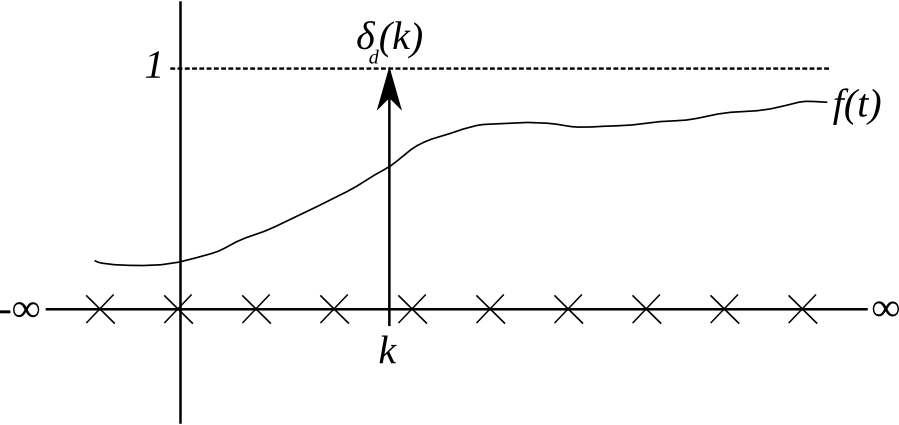
\includegraphics[width=.4\textwidth]{images/02discDeltaFn}
	\caption{Discrete-time $\delta$-function.}
	\label{fig:02discDeltaFn}
\end{figure}

\subsection{Sampling, Continuous Time}
The sampled signal, $u_s(t), t \in \mathbb{R}$, is defined as
\begin{align*}
&u_s(t) = \sum_{k=-\infty}^\infty u(t)\delta(t-k\Delta T) \\
&\int_{t=k\Delta T-\epsilon}^{k\Delta T+\epsilon} u_s(t)dt = u(k\Delta T)
\end{align*}
where $u(k\Delta T)$ is the sampled signal, $\Delta T$ is the sample time and $t=k\Delta T$, as seen in Figure \ref{fig:02samplingDeltaFn}. This lets us keep track of the information we gain or lose from the original signal. We also define the sampled signal as
$$u_d(k) = u(k\Delta T) = \int_{t=k\Delta T-\epsilon}^{k\Delta T+\epsilon} u_s(t)dt.$$
This will be useful later in comparing the Fourier transforms of discrete and continuous signals.
\begin{figure}[ht!]
	\centering
	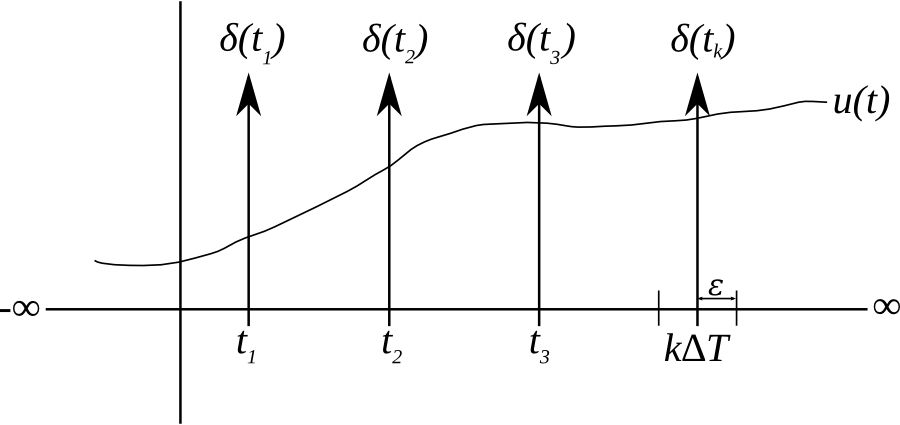
\includegraphics[width=.4\textwidth]{images/02samplingDeltaFn}
	\caption{Multiple $\delta$-functions used to sample a continuous signal.}
	\label{fig:02samplingDeltaFn}
\end{figure}

\section{Fourier Transform}
The Fourier transform involves taking a signal and decomposing it into a sum of sines and cosines. We can use Euler's formula to convert from the time to the frequency domain
$$e^{j\w t} = \cos\w t + j\sin\w t.$$
Then we can write the Fourier and inverse Fourier transforms as
\begin{align*}
U(\w) &= \tint u(t)e^{-j\w t}dt \\
u(t) &= \frac{1}{2\pi} \fint U(\w)e^{j\w t}d\w.
\end{align*}

\begin{example}
Given a signal $u(t)=\cos\wo t$ the Fourier transform is found as
\begin{align*}
U(\w) &= \tint \cos(\wo t)e^{-j\w t}dt \\
&= \tint \left(\cos(\wo t)\cos(\w t) + j\sin(-\w t)\cos(\wo t)\right)dt \\
&= \tint \left(\cos(\w t)\cos(\wo t) - j\sin(\w t)\cos(\wo t)\right)dt \\
&\text{use }\tint \sin(\w t)\cos(\wo t)dt = 0, ~ \forall \w \\
&= \tint \cos(\w t)\cos(\wo t)dt \\
&= \begin{cases} 0, & \text{if } \w \neq \wo \\ \infty, & \text{if } \w = \wo \end{cases} \\
&\Rightarrow U(\w) = \frac{1}{2} \left[\delta(\w-\wo) + \delta(\w+\wo)\right].
\end{align*}
If we want to we can go back to the time domain using the inverse Fourier transform
\begin{align*}
u(t) &= \fint U(\w)e^{j\w t}dt \\
&= \fint \frac{1}{2} \left[\delta(\w-\wo) + \delta(\w+\wo)\right] e^{j\w t}dt \\
&= \frac{1}{2}\left(e^{j\wo t} + e^{-j\wo t}\right) \\
&= \frac{1}{2}\left(2\cos\wo t\right) \\
&= \cos\wo t,
\end{align*}
which is exactly what we started with, up to a scale factor of $\frac{1}{2\pi}$ that was left out of the expression for the inverse Fourier transform.
\end{example}
$\lozenge$

\subsection{Effect of Sampling on Fourier Transform}
Notice from Figure \ref{fig:02samplingDeltaFn} that $u_s(t) = 0$ almost everywhere, with the exceptions being that $u_s(t) = \infty$ at $t=k\Delta T$. Then we have, with $t\in\mathbb{R}$ and $\w\in\mathbb{R}$,
$$u_s(t) = \sum_{k=-\infty}^\infty u(t)\delta(t-k\Delta T)$$
and
\begin{align*}
U_s(\w) &= \tint u_s(t)\emjwt dt \\
&= \tint \sum_{k=-\infty}^\infty u(t)\delta(t-k\Delta T)\emjwt dt \\
&= \sum_{k=-\infty}^\infty u(k\Delta T) e^{-j\w k\Delta T} \\
&= \sum_{k=-\infty}^\infty u_d(k) e^{-j\w k\Delta T}.
\end{align*}
This shows that an infinite sum of sampled signals is a continuous function. Also, since we know that $e^{-j\w k\Delta T} = \cos(\w k\Delta T) - j\sin(\w k\Delta T)$, then we can say that $e^{-j\w k\Delta T}$ has periodicity with $\w_s = \frac{2\pi}{\Delta T}$, where $\w_s$ is known as the sampling frequency and has units of $rad/s$. This lets us write
\begin{align*}
U_s(\w) &= U_s(\w+n\w_s) \text{, where } \w_s = \frac{2\pi}{\Delta T} \text{, } n\in\mathbb{Z} \\
\Rightarrow U_s(\w) &= U_s(\w+\frac{2\pi}{\Delta T}) \text{, } n=1 \\
U_s(\w) &= -\overline{U_s(\w)}.
\end{align*}
$\mathbb{Z}$ is the set of natural numbers and $\overline{(\cdot)}$ represents the complex conjugate of $(\cdot)$. Remember that $U_s(\w)$ is the Fourier transform of $u_s(t)$. Using the properties of the Fourier transform it is only necessary to know a small segment of the function, the rest can be automatically duplicated as shown in Figure \ref{fig:02sin}, where knowledge of the function in the range $[0,\frac{2\pi}{\Delta T}]$ is sufficient to recreate the entire function shown.
\begin{figure}[ht!]
	\centering
	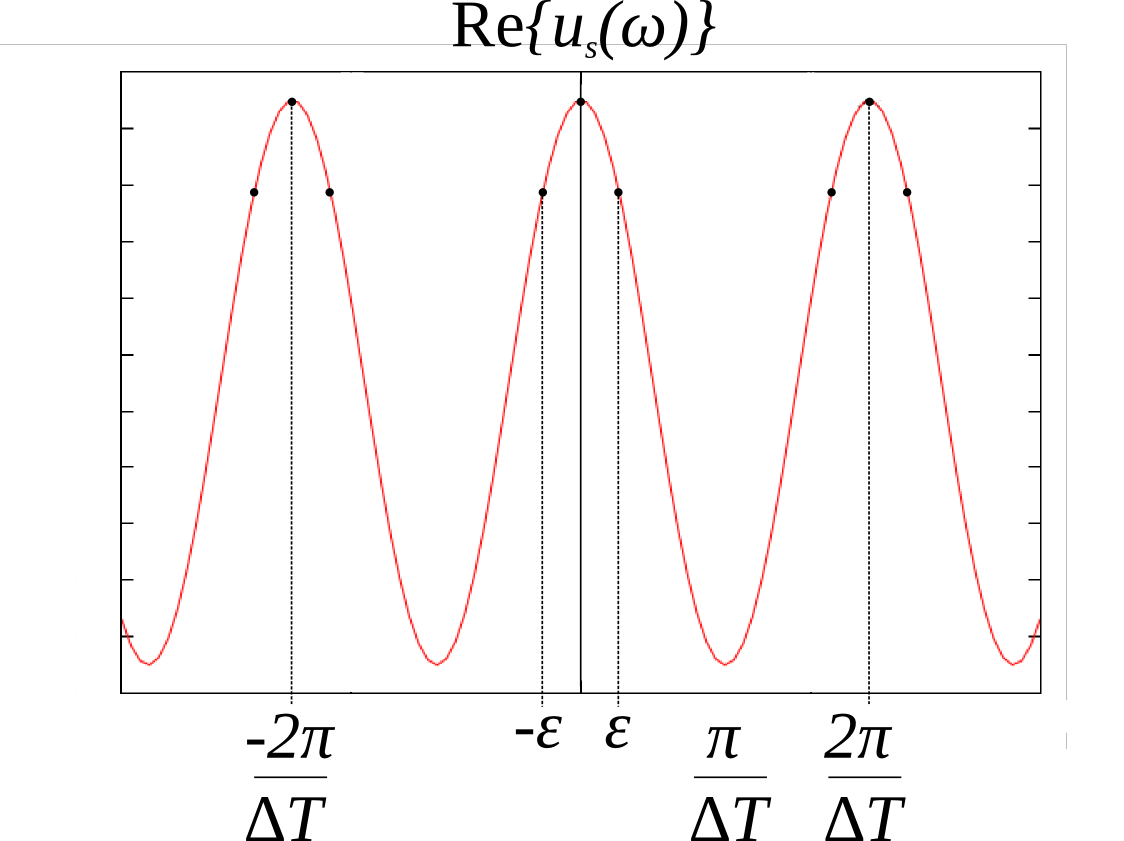
\includegraphics[width=.3\textwidth]{images/02sin}
	\caption{Illustration of using Fourier transform rules to automatically fill in function.}
	\label{fig:02sin}
\end{figure}

The result of looking at $\text{Re}\{U_s(\w)\}$ is that the signal, after going through a Fourier transform, is periodic over the range $[0, \frac{2\pi}{\Delta T}]$ and that the complex conjugate of the signal is the same as the original signal. Thus, it is sufficient to compute the Fourier transform \textit{only} over the range $[0, \frac{\pi}{\Delta T}]$. This sampling frequency is known as the Nyquist frequency, $\w_N = \frac{\w_s}{2} = \frac{\pi}{2}$, and has units of $rad/s$.

One of the drawbacks of sampling a continuous-time signal is that information about higher frequencies is lost. This can be seen by looking at a sinusoidal function. If $f(t) = \sin(\w t)$ and samples are taken at $\w_N = \frac{\w t}{2}$, then $f(t)$ will look like $f(t) = 0$ when sampling. That is how information is lost. Figure \ref{fig:02lowSampleRate} shows that if the signal is a sine wave that is only sampled at the points indicated the captured signal will look like a line with zero slope and zero magnitude.
\begin{figure}[ht!]
	\centering
	\includegraphics[width=.3\textwidth]{images/02lowSampleRate}
	\caption{Sampling of a sine wave at a low sampling rate.}
	\label{fig:02lowSampleRate}
\end{figure}

\subsection{Relation between Original and Sampled Signal}
Given
$$U_s(\w) = \w_s \sum_{k=-\infty}^\infty U(\w-k\w_s), \w_s = \frac{2\pi}{\Delta T}$$
where $U(\w-k\w_s)$ is the original signal shifted by $\w_s$, we can see how high frequency information is lost as shown in Figure \ref{fig:02freqResp}. The sampled signal has a higher magnitude than the original signal throughout most of the range.
\begin{figure}[ht!]
	\centering
	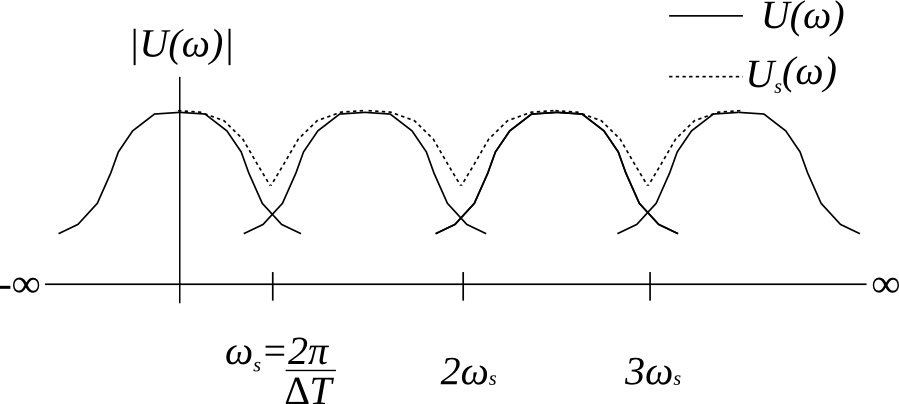
\includegraphics[width=.4\textwidth]{images/02freqResp}
	\caption{Sampling of a sine wave at a low sampling rate.}
	\label{fig:02freqResp}
\end{figure}

\subsection{Aliasing}
After a Fourier transform is applied low frequencies are about the same but high frequencies appear to have a larger magnitude compared to the original signal. This is due to shifting by $\w_s$ and is called aliasing, as seen in Figure \ref{fig:02aliasingSines}.
\begin{figure}[ht!]
	\centering
	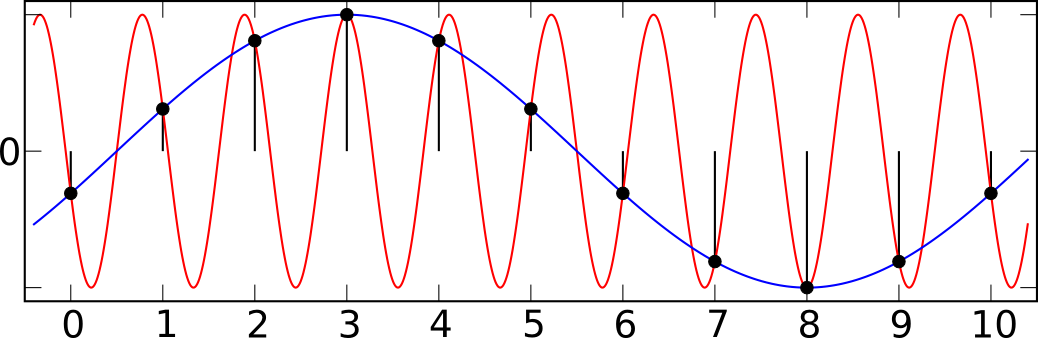
\includegraphics[width=.5\textwidth]{images/02aliasingSines}
	\caption{Effects of aliasing with original and sampled signal.}
	\label{fig:02aliasingSines}
\end{figure}

To remove artifacts due to aliasing we need to sample at $\w_s = 2\cdot\w_N$. If it is not possible to sample at $\w_s = 2\cdot\w_N$ because of hardware limitations or some other factor then an anit-aliasing filter is needed. For example, if $\w_N = 100 Hz$, then the anti-aliasing filter should use a cut-off of $< 50 Hz$, which will act as a low-pass filter in order to remove the artifacts associated with high frequencies.
\begin{figure}[ht!]
	\centering
	\includegraphics[width=.25\textwidth]{images/02aafilter}
	\caption{Block diagram of estimator with anti-aliasing filter.}
	\label{fig:02aafilter}
\end{figure}

\subsection{Discrete-Time Fourier Transform (DTFT)}
A DTFT is defined, for $\w\in\mathbb{R}$, by
\begin{align*}
U_\infty(\w) &= \tint u_s(t)\emjwt dt \\
&= \sum_{k=-\infty}^\infty u(k\Delta T) e^{-j\w k\Delta T} \\
&= \sum_{k=-\infty}^\infty u_d(k) e^{-j\w k\Delta T}
\end{align*}
where $u_d(k)$ represents the discrete time samples used to compute the continuous-time Fourier transform, $U_\infty(\w)$. Note that we only need to evaluate $\w\in[0, \frac{\pi}{\Delta T}]$.

\subsection{Finite Time Fourier Transform (FTFT)}
A FTFT is defined, for $\w\in\mathbb{R}$, by
$$U_N(\w) = \sum_{k=0}^{N-1} u_d(k) e^{-j\w k\Delta T}.$$

\subsection{Properties of Fourier Transforms}
Some useful properties of Fourier transforms are
\begin{itemize}
\item $U_\infty(\w) = U_\infty(\w + n\cdot \frac{2\pi}{\Delta T})$
\item $\overline{U_\infty(-\w)} = U_\infty(\w)$
\item If $u_d(k) = u_d(-k)$ then the $\sin$'s cancel out leaving $U_\infty(\w)\in\mathbb{R}$. This is known as a ``symmetric discrete-time signal around $0$''.
\item If $u_d(k) = -u_d(-k)$ then the $\cos$'s cancel out and $\text{Re}\lbrace U_\infty(\w)\rbrace = 0$.
\item If $u(t)$ and thus $u_d(k)$ is periodic with period $T=N\Delta T$, then $U_\infty(\w) = \frac{2\pi}{T}U_N(\w) \sum_{l=-\infty}^\infty \delta(\w-l\frac{2\pi}{T})$.
\end{itemize}
When the signal is periodic there are several other important properties. The finite time DTFT multiplied by an infinite sum of delta functions results in spikes at the points where there is a sinusoid in the signal. Recall that $U_\infty(\w)=0$ almost everywhere except at those frequencies that are multiples of $l\cdot \frac{2\pi}{T}$.

Then the sampled version of the finite time DTFT is
$$\int_{\w=l\cdot \frac{2\pi}{T}-\epsilon}^{l\cdot \frac{2\pi}{T}+\epsilon} U_\infty(\w)d\w
= \frac{2\pi}{T}U_N(l\cdot \frac{2\pi}{T}).$$
This shows that we only need to compute the finite time DTFT for the range $\w\in[0,\frac{\pi}{T}]$, and even then we only need to compute at the discrete frequencies of $l\cdot\frac{2\pi}{T}$ on that range.

\subsection{Discrete Fourier Transform (DFT)}
The discrete, or ``sampled'', Fourier transform is defined as
$$U_N(l) = \sum_{k=0}^{N-1} u_d(k) e^{-jl\frac{2\pi}{T}k\Delta T}$$
and we can go the other direction using
$$u_d(k\Delta T) = \frac{1}{T} \sum_{l=0}^{N-1} U_N(l) e^{jl\frac{2\pi}{T}k\Delta T}.$$
These are the functions used to compute Fourier transforms in \textsc{Matlab} using the \texttt{fft} command.

\subsection{Measurement Resolution and Implied Periodicity}
The resolution in the time domain is $\Delta T$, with units of $s$. The resolution in the frequency domain is $\frac{2\pi}{T}$, with units in $rad/s$. Note that $T=N\cdot\Delta T$. The resolution in the frequency domain is a function of the number of samples \textit{and} the sampling time. This makes sense because  we need to sample signals longer in order to capture the low-frequency portions of the signal.

$N$ points in the time domain (which only have $\text{Re}$ parts and no $\text{Im}$ parts) results in $\frac{N}{2}$ points in the frequency domain. Those $\frac{N}{2}$ points in the frequency domain are in the range $[0,\frac{\pi}{\Delta T}]$, and each of those points has a real and an imaginary part.

An important point to notice is that once a signal is sampled to generate $U_N(\w)$ at $U_N(\frac{2\pi}{T}\cdot l)$ there is an implicit assumption made that the original signal, $u(t)$, was periodic!


\end{document}

%%%%%%%%%%%%%%%%%%%%%%%%%%%%%%%%%%%%%%%%%%%%%%%%%%%%%%%%%%%%%